\section{Variability Mechanisms}

\subsection{Main Variability Aspects}
For FridgeIO the main variability aspects is a bit limited, but includes:

\begin{enumerate}
    \item \textbf{User Management}
    \begin{itemize}
        \item \hyperref[fig:FridgeIOLogin]{Login page for authentication}
        \item Registration of new users
        \item Editing and deleting user accounts
    \end{itemize}

    \item \textbf{Security}
    \begin{itemize}
        \item Password hashing and salting for credential protection
    \end{itemize}

    \item \textbf{API}
    \begin{itemize}
        \item Supports GET, POST, PUT and DELETE HTTP Methods
    \end{itemize}

    \item \textbf{Inventory Management}
    \begin{itemize}
        \item Add custom food items with expiration dates
        \item Edit items
        \item Remove items from inventory
        \item Mark items as favorites
    \end{itemize}

    \item \textbf{Recipe Management}
    \begin{itemize}
        \item Create custom recipes with ingredients linked to the inventory
        \item Edit existing recipes
        \item Delete recipes
    \end{itemize}
\end{enumerate}

These variability aspects are a bit basic, and most features are tightly coupled to the FridgeIO context, making them difficult to reuse in other types of software. FridgeIO was originally planned to be a modular project where we could easily expand or improve separate parts in the future. In the end it we failed at the goal to make it modular. The most modular elements we made was the React components we created for the web interface, such as the  \hyperref[fig:Components]{login form, recipe page, and settings page}. These components mainly help with readability on the frontend pages but was difficult to integrate with backend functionality. Easier to read, still not modular.

\begin{figure}[h]
    \centering
    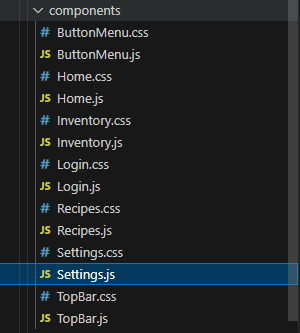
\includegraphics[width=0.5\linewidth]{images/Components.png}
    \caption{React components used in FridgeIO}
    \label{fig:Components}
\end{figure}

\subsection{Variability aspects implementation}
\begin{enumerate}
    \item \textbf{User Management}

    User management variability (Account creation, login, account deletion) is implemented through runtime binding, the user decides which action is performed when interacting with the application. In practice, these features are implemented as separate React components on the frontend and backed by API calls to the backend. This makes it a composition-based approach, each component is included or not depending on navigation, so not by conditional code.
    
    From a variability mechanism perspective, this follows a framework + component model: React provides the framework in the form of control flow and extension points, while user management actions are implemented as reusable components plugged into it.
    
    \item \textbf{Security}
    
    Security variability is less present but still present. Password hashing and salting is an constant mandatory feature, so there is no compile-time or run-time feature selection. It is implemented directly in the backend using \textbf{bcrypt}, a Golang module. Since all deployed products include the hashing logic without modular toggling, so it's a fixed implementation.  
    
    In terms of variability implementation, it is closer to parameters, since each password is hashed with a unique random salt generated by the \textbf{bcrypt} module. No variability between hashing algorithms exists in the current prototype, but in principle this could be extended using the Strategy pattern to allow alternative algorithms.  

        
    \item \textbf{API}
    
    For the API variability comes because each HTTP method exposes a different behavior, but all methods are present in the codebase. This is a case of annotation-based variability, the methods are coded within the same API module, and the variability is resolved at run-time when the frontend chooses which method to call.
    
    The implementation mechanism here is language-based variability. Each method corresponds to a different route handler in Golang. Unlike frameworks, this variability is “hard-wired” into the backend. A more modular approach could use the Template Method pattern, where the core request pipeline is fixed, but specific behaviors like GET or POST are made dynamically.
    
    \item \textbf{Inventory Management}
    
    The Inventory features are implemented as React components combined with backend API calls. This is a composition-based variability mechanism, since inventory actions are implemented as separate modules/components rather than controlled by annotations. The variability is resolved at run-time, depending on what the user does.
    
    The Inventory management page can fit the Decorator pattern. A inventory object like a food item can be “decorated” with additional attributes like expiration date or favorite status. These extra features are optional, giving some flexibility to the data model without changing the entire system.
    
    \item \textbf{Recipe Management}
    
    Like inventory, this is implemented as composition-based run-time variability. Recipes are stored in the same backend but managed through separate API endpoints and frontend components. Users decide at run-time whether to create or modify recipes, so the variability binding is late.
    
    If this got expanded on, this could use the Template Method pattern. It could be a general “recipe handler” and could define the structure with like title, ingredients and steps, while subclasses/extensions handle optional features like auto-removal of ingredients or recipe sharing. Another alternative could be using the Decorator pattern as mentioned with Inventory management. With some changes like with like sharing or tagging we could try to dynamically layer that on top of the original functionality. But currently, all recipe functionality is implemented in a straightforward modular fashion, without explicit design patterns. but could also fit the decorator pattern with a little more change.

\end{enumerate}